% !TeX spellcheck = en_US
\section{APPROACHES}
\label{sec:approaches}

In general, the task of text detection consists of recognizing the required text from images. In some tasks, like ours, it is required to find all the fragments of text within a page, but for other purposes reading the entire document is not needed, rather the objective is extracting a piece of information within it (e.g. credit card number, amount and date from bills, etc). The main reason why this problem, and, in general, every object detection problem, can not be solved by a standard convolutional network followed by a fully connected layer is that, since the number of occurrences of objects (characters in our case) is not fixed, the length of the output layer is variable. A naive solution to this issue would be taking different regions of interest from the image and use a CNN to classify the objects within those regions. The problem with this approach is that the objects of interest might have different spatial locations within the image and different aspect ratios. Hence, a select over a huge number of regions would be needed, and this may not be computationally affordable. Therefore, a number of algorithms have been developed to balance computational costs and time without renouncing to good detection performances.

\subsection{Region-based}
\label{ssec:regionbased}

Region-based methods work by finding all the regions which may contain an object, and then passing those regions to a classifier which defines the locations of the required objects. In order to bypass the problem of selecting a huge number of regions, the R-CNN uses a method that implies a selective search to extract about 2000 regions from the image, which are called region proposals. These candidate regions are resized into square images and fed into a convolutional neural network that produces a 4096-dimensional feature vector as output. The CNN acts as a feature extractor and the extracted features are then fed into an SVM to classify the presence of the object within that candidate region proposal \cite{Gandhi2018}. A simplified overview of this approach is presented in figure \ref{fig:rcnn}.

\begin{figure}[h]
	\caption{Overview of the R-CNN object detection system \cite{Gandhi2018}.}
	\centering
	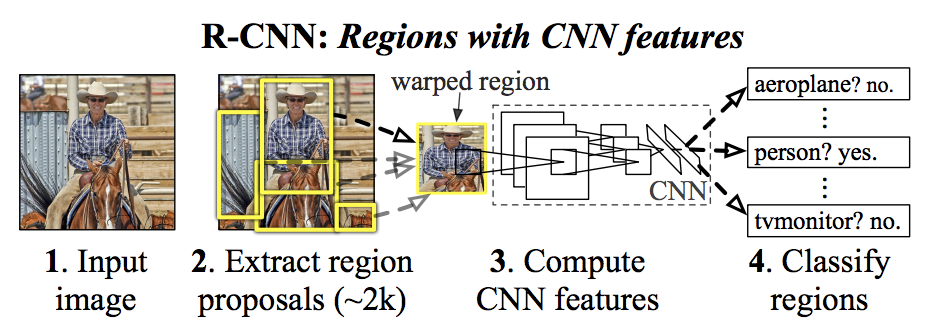
\includegraphics[width=0.5\textwidth]{approaches/RCNN.png}
	\label{fig:rcnn}
\end{figure}

Note that this approach is considered more accurate, but it is quite slow if compared with other methods. It takes a huge amount of time to train the network as the model needs to classify 2000 region proposals per image. Furthermore, the selective search algorithm is a fixed algorithm. Therefore, no learning is happening at that stage, which could lead to the generation of bad candidate region proposals. However, improvements have been shown in subsequent research. The Fast R-CNN algorithm solved some of the major drawbacks of R-CNN t	o build a faster object detection system: the approach is similar to the R-CNN algorithm, but instead of feeding the region proposals to the CNN, the whole input image is fed to the CNN to generate a convolutional feature map \cite{Girshick2015-ay}. The Faster R-CNN algorithm then eliminates the selective search algorithm and lets the network learn the region proposals by itself \cite{Ren2017-fu}.

\subsection{Single shot}
\label{ssec:singleshot}

Single shot detectors predict both the bounding box and the class of an object at the same time. Being a single step process, it is much faster and indicated for real-time object detection. Instead of having a network produce proposals, the single shot approach implies the exploitation of a set of predefined boxes to look for objects. In order to understand what is in an image, the input is fed through a standard convolutional network to build a rich feature representation of the original image. This part of the architecture is the "backbone" network, which is usually pre-trained as an image classifier to more cheaply learn how to extract features from an image. After pre-training the backbone architecture as an image classifier, its last few layers are removed, so that its output consists of a collection of stacked feature maps which describe the original image in a low spatial resolution but in a high feature (channel) resolution. In order to detect an object, another convolutional layer is added, and the kernel parameters must be learned, which combine the context of all the feature maps of the object in order to produce an activation corresponding with the grid cell which contains it \cite{Jordan2018}. This process is showed in figure \ref{fig:ssd} \\

\begin{figure}[h]
	\caption{Combination of the feature maps to produce an activation in the grid cell responsible for detecting an object in a single shot detector \cite{Jordan2018}.}
	\centering
	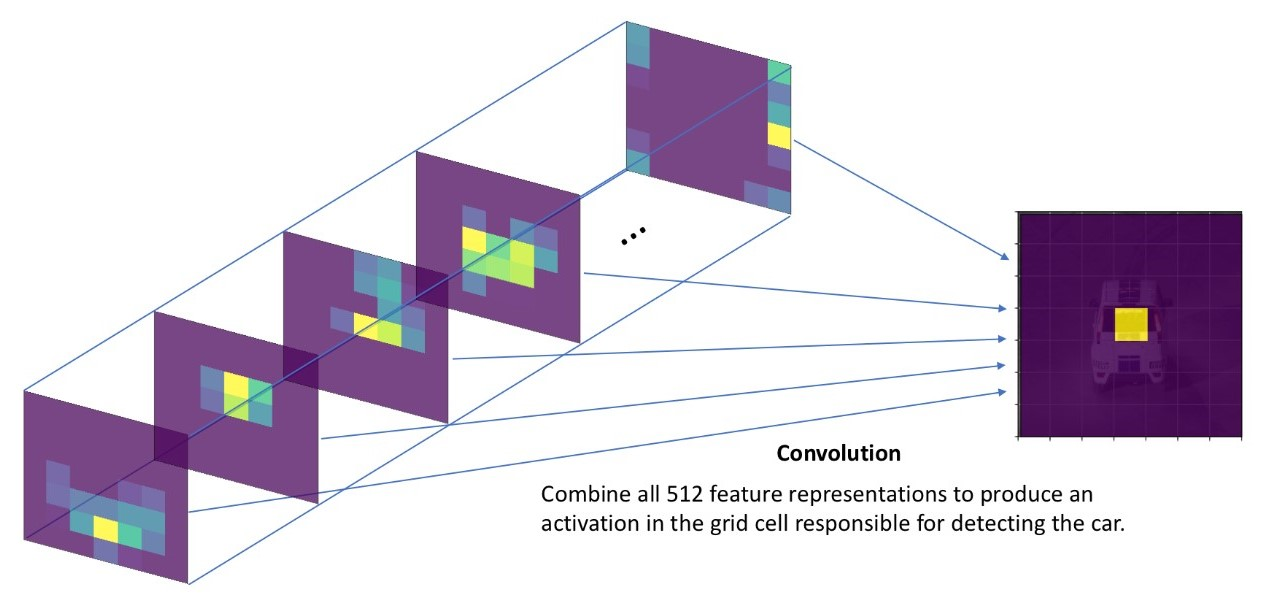
\includegraphics[width=0.5\textwidth]{approaches/SSD.jpg}
	\label{fig:ssd}
\end{figure}

Because of the convolutional nature of the detection process, multiple objects can be detected in parallel, substantially increasing the overall speed of the algorithm. However, the method also ends up predicting for a large number of grid cells where no object is found. Although the majority of the redundant bounding boxes could be filtered out by selecting a proper confidence threshold, multiple high-confidence predictions describing the same object may persist. Thus, a method is needed for removing redundant object predictions such that each object is described by a single bounding box. To accomplish this, a technique known as non-maximum suppression is used. At a high level, this technique will look at much overlapping bounding boxes and suppress all the predictions except the one with the highest confidence value. The strategy is schematized in figure \ref{fig:nms}.

\begin{figure}[h]
	\caption{Non-maximum suppression strategy \cite{Jordan2018}.}
	\centering
	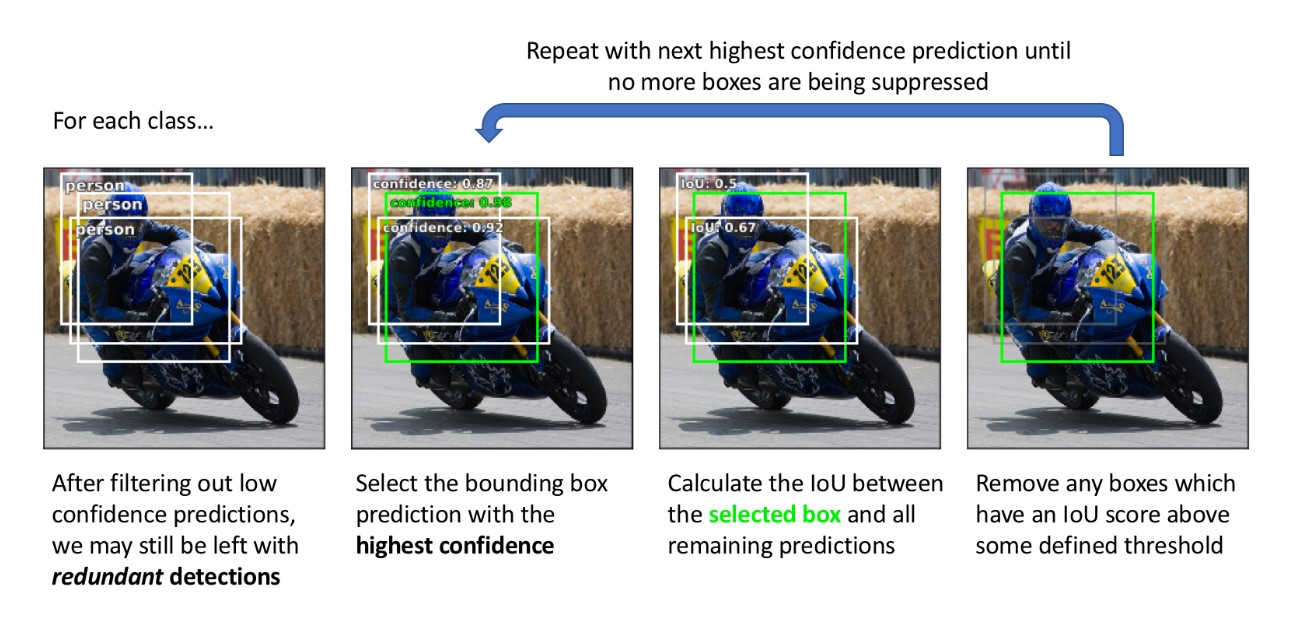
\includegraphics[width=0.5\textwidth]{approaches/nms.jpg}
	\label{fig:nms}
\end{figure}

One of the most popular Single Shot detectors is the YOLO (You Only Look Once) network. The original YOLO network (YOLO v1) \cite{Redmon2015-cy} uses a modified GoogLeNet as the backbone network. Later on, \citeauthor{Redmon2016-ad}\cite{Redmon2016-ad} proposed a new model named DarkNet-19 (YOLO v2) which follows the general design of $3\times3$ filters, doubling the number of channels at each pooling step; 1x1 filters are also used to periodically compress the feature representation throughout the network. Finally, in a different paper, \citeauthor{Redmon_undated-wa}\cite{Redmon_undated-wa} introduces a new, larger model named DarkNet-53 (YOLO v3) which offers improved performance over its predecessor. All of these models were first pre-trained as image classifiers before being adapted for the detection task, adapting the classification network for detection simply consists of removing the last few layers of the network and adding a convolutional layer with $B(5+C)$ filters to produce the NNB bounding box predictions. The first iteration of the YOLO model directly predicts all the four values which describe a bounding box. The x and y coordinates of each bounding box are defined relative to the top left corner of each grid cell and normalized by the cell dimensions such that the coordinate values are bounded between 0 and 1. The width and height of the boxes are user-defined, such that the model predicts the square-root width and height, and an L2 loss is applied during training. This formulation was later revised to introduce the concept of a bounding box prior: rather than expecting the model to directly produce unique bounding box descriptors for each new image, the user will define a collection of bounding boxes with varying aspect ratios which embed some prior information about the shape of objects that are to be expected in the examples. Rather than directly predicting the bounding box dimensions, the task is reformulated in order to simply predict the offset from the bounding box prior dimensions such that it is possible to fine-tune the predicted bounding box dimensions. This reformulation makes the prediction task easier to learn.